%% ============================================================
%%  EC8070 – Research Project III
%%  AI-Based Optimized Energy Utilization System Using
%%  Edge Computing Controllers
%%
%%  Compile with:  pdflatex research_paper.tex
%%  Requires:      IEEEtran.cls  (bundled with most TeX distros)
%% ============================================================
\documentclass[conference]{IEEEtran}

%% ---- Packages -----------------------------------------------
\usepackage[T1]{fontenc}
\usepackage[utf8]{inputenc}
\usepackage{amsmath}
\usepackage{graphicx}
\usepackage{booktabs}
\usepackage{array}
\usepackage{url}
\usepackage{microtype}
\usepackage{cite}
\usepackage{hyperref}
\hypersetup{
  colorlinks = false,
  pdfborder  = {0 0 0}
}

%% ---- Title & Authors ----------------------------------------
\begin{document}

\title{AI-Based Optimized Energy Utilization System Using\\Edge Computing Controllers}

\author{%
  \IEEEauthorblockN{%
    E.M.I.~Indrajith$^{1}$\IEEEauthorrefmark{1}\quad
    H.P.M.~Hettiarachchi$^{2}$\IEEEauthorrefmark{2}%
  }
  \IEEEauthorblockA{%
    \textit{Department of Electrical and Information Engineering}\\
    \textit{Faculty of Engineering, University of Ruhuna}\\
    Galle, Sri Lanka\\
    $^{1}$Reg.~No.:~2021/E/035\quad
    $^{2}$Reg.~No.:~2021/E/051
  }
  \medskip
  \IEEEauthorblockN{%
    \textit{Supervisor:}~Dr.~A.~Kaneswaren\quad
    \textit{Co-Supervisor:}~Mr.~Y.~Pirunthapan%
  }
  \IEEEauthorblockA{%
    \textit{Department of Electrical and Information Engineering}\\
    \textit{Faculty of Engineering, University of Ruhuna}\\
    Galle, Sri Lanka
  }
}

\maketitle

%% ---- Abstract -----------------------------------------------
\begin{abstract}
Rising household electricity costs and inefficient appliance usage
present a growing challenge for domestic energy management.
This paper presents an AI-based energy utilization system that
combines Long Short-Term Memory (LSTM) neural network forecasting
with an edge-deployed Large Language Model (LLM) agent to
intelligently predict and optimize household appliance schedules.
The LSTM model forecasts 24-hour power consumption patterns
for five appliances—washing machine, heater, air conditioner
(AC), vehicle charger, and vacuum cleaner—using historical
minute-level telemetry.
Predicted states are passed to an optimization agent that
retrieves live Time-of-Use (TOU) electricity tariffs via MQTT,
real-time weather data from the Open-Meteo API, and user
preferences stored in Firebase Firestore.
A locally-hosted Llama~3.2 model (via Ollama) then generates
optimized schedules, which are subsequently corrected by
deterministic post-processing rules that enforce hard constraints
on peak-hour usage and preserve total appliance runtime.
Experimental results on simulated Sri Lankan domestic tariff data
demonstrate average per-cycle cost reductions exceeding 40\%,
achieved without compromising user-specified appliance runtime
requirements.
The fully edge-native architecture ensures low latency, user
privacy, and offline operational capability, making the system
practical for deployment on resource-constrained hardware such
as a Raspberry Pi.
\end{abstract}

\begin{IEEEkeywords}
Edge Computing, Energy Optimization, LSTM, Time-of-Use Pricing,
LLM Scheduling, Demand Response, Smart Home, IoT
\end{IEEEkeywords}

%% ============================================================
\section{Introduction}
\label{sec:intro}
%% ============================================================

Household electricity demand in developing nations has grown
consistently over the past decade, driven by rising appliance
penetration and urban electrification \cite{zhu2022green}.
In Sri Lanka, the Ceylon Electricity Board operates a three-band
domestic Time-of-Use (TOU) tariff structure: an off-peak band at
LKR~21\,kWh$^{-1}$ (22:30–05:30), a day band at
LKR~35\,kWh$^{-1}$ (05:30–18:30), and a peak band at
LKR~67\,kWh$^{-1}$ (18:30–22:30).
Without intelligent scheduling, households routinely operate
high-wattage appliances during the expensive peak window,
incurring unnecessarily high bills.

Traditional energy management systems rely on fixed timers or
rule-based heuristics that fail to adapt to changing consumption
patterns, real-time pricing, or ambient environmental conditions
\cite{lekidis2023edge}.
Recent advances in deep learning, particularly LSTM-based
time-series forecasting, have improved the accuracy of appliance-level
energy prediction \cite{severiche2025forecasting,zhao2024residential}.
However, most state-of-the-art approaches stop at prediction;
they do not close the control loop by translating forecasts into
actionable, optimized schedules.

The research gap this work addresses is the integration of
forecasting with real-time, context-aware optimization at the edge.
While cloud-based demand-response platforms exist, they introduce
latency, dependency on connectivity, and privacy concerns
\cite{zawish2023energy,ali2023iot}.
Edge AI approaches that can run entirely on local hardware remain
underexplored for fine-grained, appliance-level domestic scheduling.

\textbf{Aim:} To develop an edge-deployable AI system that predicts
household appliance usage and automatically re-schedules operations
to cheaper off-peak tariff bands, minimizing electricity cost while
preserving user-specified appliance runtime requirements.

\textbf{Objectives:}
\begin{enumerate}
  \item Train an LSTM model on historical appliance power data to
        generate 24-hour ON/OFF state predictions.
  \item Design an edge agent that ingests live TOU tariffs, weather
        forecasts, and user preferences to generate context-aware
        optimized schedules via a local LLM.
  \item Enforce hard scheduling constraints through deterministic
        post-processing rules.
  \item Validate cost savings quantitatively and expose results
        through a Firebase-backed Flutter mobile application.
\end{enumerate}

The key contribution of this work is a novel hybrid pipeline—LSTM
prediction followed by LLM-assisted scheduling with rule-based
post-processing—that operates entirely on an edge controller,
enabling real-time, privacy-preserving household energy optimization.

%% ============================================================
\section{Methodology}
\label{sec:method}
%% ============================================================

The system is organized as a two-stage pipeline as illustrated in
Fig.~\ref{fig:arch}.

\begin{figure}[t]
  \centering
  %% Replace the rule below with \includegraphics once you have a figure:
  %% \includegraphics[width=\columnwidth]{figures/system_architecture.pdf}
  \rule{\columnwidth}{0.4pt}\\[4pt]
  \small\textit{%
    Stage~1 (LSTM Predictor): MQTT sensor data $\rightarrow$
    circular buffer $\rightarrow$ MinMaxScaler $\rightarrow$
    LSTM model $\rightarrow$ binarizer $\rightarrow$
    \texttt{appliance\_data.txt}.\\[4pt]
    Stage~2 (Optimization Agent): \texttt{appliance\_data.txt} +
    MQTT TOU tariffs + Open-Meteo weather + user preferences
    $\rightarrow$ Llama~3.2 (Ollama) $\rightarrow$ post-processing
    $\rightarrow$ Firestore $\rightarrow$ Flutter app.
  }\\[4pt]
  \rule{\columnwidth}{0.4pt}
  \caption{End-to-end system architecture.}
  \label{fig:arch}
\end{figure}

\subsection{Stage 1 — LSTM-Based Appliance State Prediction}

\subsubsection{Data Collection and Preprocessing}
Minute-level power readings for five appliances
(WashingMachine, Heater, AC, VehicleCharger, VacuumCleaner)
are published by smart-home sensors to a local MQTT broker
on topic \texttt{home/power}.
The predictor (\texttt{Run\_LSTM.py}) maintains a circular
buffer of 1\,464 samples, corresponding to approximately
24~hours of one-sample-per-minute telemetry.
At startup, the buffer is bootstrapped with realistic synthetic
samples generated by \texttt{generate\_dummy\_sample()}, which
simulates per-appliance usage patterns (e.g., the vehicle charger
operates a single 5-hour session overnight at 80–100\% of rated
3\,500\,W).
All values are normalized to $[0,1]$ using a \texttt{MinMaxScaler}
fitted on training data and persisted as \texttt{scaler.pkl}.

\subsubsection{Model Architecture and Training}
A sequential LSTM network is constructed in TensorFlow/Keras
with the following topology:
\[
  \texttt{LSTM}(64\text{ units}) \;\rightarrow\;
  \texttt{Dense}(5\text{ outputs})
\]
Inputs are overlapping sliding windows of length
$T_s = 24$ consecutive normalized samples
(shape: $[N, 24, 5]$), where the target output is the
next time-step's power for all five appliances simultaneously.
The Adam optimizer \cite{goodfellow2016deep} with default
learning rate $\alpha = 10^{-3}$ and mean squared error (MSE)
loss is used.
The model is trained on historical data with a 70/15/15
train/validation/test split and saved as
\texttt{my\_lstm\_model.keras}.

\subsubsection{Prediction and Binarization}
Every 30 new MQTT messages, \texttt{predict\_on\_buffer()} creates
all valid sliding windows from the buffer, runs batch inference,
and inverse-transforms predictions back to watts.
The resulting minute-level predictions are aggregated into
24 hourly averages.
A dynamic threshold converts each hourly average into a binary
ON/OFF state:
\[
  \text{State}_h =
  \begin{cases}
    1 & \text{if } \bar{P}_h \;\geq\; \tau \cdot \max_h(\bar{P}_h) \\
    0 & \text{otherwise}
  \end{cases}
\]
where $\tau = 0.6$ for AC, Heater, and WashingMachine
(variable-usage appliances) and $\tau = 0.8$ for VehicleCharger
and VacuumCleaner (distinct ON/OFF profile appliances).
The 24-element binary arrays are written to
\texttt{appliance\_data.txt} as input for Stage~2.

\subsection{Stage 2 — Edge Optimization Agent}

\subsubsection{Context Gathering}
At each optimization cycle, \texttt{agent.py} collects three
live data sources:
\begin{itemize}
  \item \textbf{TOU tariffs} via MQTT topic
        \texttt{power/tou\_domestic} on the public broker
        \texttt{test.mosquitto.org}.
        The JSON payload specifies price and time range for each
        of the three bands (day, peak, off-peak).
  \item \textbf{Weather forecast} via the Open-Meteo REST API
        for Colombo (lat.~6.9271°\,N, lon.~79.8612°\,E),
        returning hourly temperature (°C) and relative humidity
        (\%) for the next 24~hours.
  \item \textbf{User preferences} parsed from a natural-language
        command (e.g., ``Allow AC\_Power ON during peak hours'')
        and stored in Firebase Firestore.
\end{itemize}

\subsubsection{LLM-Assisted Scheduling}
When the flag \texttt{USE\_LLM\_FOR\_SCHED = True},
the agent invokes Llama~3.2 (\texttt{llama3.2:latest})
via a local Ollama daemon at temperature $= 0.0$ to
eliminate stochastic variation.
A weather-aware system prompt is generated by
\texttt{build\_system\_prompt()}, encoding the following rules:
\begin{itemize}
  \item \textbf{AC}: If temperature $\geq 28\,^\circ\text{C}$
        or humidity $\geq 80\%$, those hours are flagged as
        \emph{hot\_hours}; the LLM is instructed to keep
        AC ON during those periods.
  \item \textbf{Heater}: If temperature $\leq 20\,^\circ\text{C}$,
        flagged as \emph{cold\_hours}; the LLM prioritizes
        heater operation then.
  \item \textbf{All appliances}: Unless peak usage is explicitly
        permitted, the LLM must avoid scheduling any appliance
        in the peak band.
\end{itemize}
The LLM returns one updated 24-element binary array per appliance;
\texttt{extract\_first\_array()} uses a regular-expression parser
to strip markdown artefacts from the raw model output.
If Ollama is unavailable, the original LSTM-predicted schedule
is used as a fallback.

\subsubsection{Deterministic Post-Processing}
Even with temperature $= 0.0$, the LLM may occasionally violate
constraints. Two deterministic correctors are applied sequentially:

\textbf{1. Peak Redistribution} (\texttt{redistribute\_peak\_violations}):
For any appliance where peak usage is not permitted, all
ON-hours within the peak window are set to 0 and greedily
reassigned to the cheapest available non-peak hours
(off-peak preferred over day band).

\textbf{2. Runtime Enforcement} (\texttt{enforce\_required\_ons\_improved}):
The total number of ON-hours must equal the predicted
baseline exactly.
If the count is low, missing ONs are inserted into
off-peak slots first; if high, excess ONs are removed from
day slots first.

\subsubsection{Cost Calculation and Output}
Per-appliance hourly cost is computed as:
\begin{equation}
  C_{\text{appliance}} = \sum_{h=0}^{23}
    s_h \cdot P_{\text{kWh}} \cdot r_h
  \label{eq:cost}
\end{equation}
where $s_h \in \{0,1\}$ is the schedule state,
$P_{\text{kWh}}$ is rated hourly energy consumption (kWh),
and $r_h$ is the TOU rate (LKR\,kWh$^{-1}$) at hour $h$.
Savings are reported as $C_{\text{original}} - C_{\text{optimized}}$
for each appliance and in aggregate.
Results are written to \texttt{output.txt} (schedules) and
\texttt{output\_explanations.txt} (rationale and savings),
then uploaded to Firebase Firestore under the document
\texttt{analysis/latest}.

\subsubsection{Mobile Application}
A Flutter mobile application fetches the optimized schedules
and cost-savings summary from the Firestore-backed Flask API
(\texttt{server\_firestore.py}, port~8080).
The \textit{Predictions Page} refreshes every 30~minutes,
displaying per-appliance ON/OFF schedules, original vs.\
optimized costs, and total daily savings.

\subsubsection{Ethical Considerations}
All power consumption data used during development are synthetic
or anonymized; no personally identifiable information is
collected, stored, or transmitted.
The system's source code and configuration are fully documented
to ensure reproducibility.

%% ============================================================
\section{Results}
\label{sec:results}
%% ============================================================

\subsection{LSTM Prediction Performance}

The LSTM model (\texttt{LSTM}(128) $\rightarrow$ \texttt{Dense}(5))
was trained for 50~epochs with a batch size of~32 on a dataset of
five appliance power columns sampled at one-minute intervals
(70\% train / 20\% validation / 10\% test split, \texttt{shuffle=False}
to preserve temporal order).
Mean Squared Error (MSE) was used as the loss function and
optimized with Adam ($\alpha = 10^{-3}$).

Fig.~\ref{fig:loss} shows the training and validation loss curves
recorded across all 50~epochs.
Both curves decrease sharply in the first 10~epochs, reflecting
rapid weight convergence, then plateau smoothly without diverging.
Training loss fell from an initial value of approximately
$\mathcal{L} \approx 0.0095$ at epoch~1 to
$\mathcal{L} \approx 0.0023$ by epoch~50.
Validation loss tracked the training curve closely throughout,
with the gap between the two remaining below 5\% at epoch~50,
indicating that the model generalized well and did not overfit to
the training data.
The model was subsequently evaluated on the held-out test split
using \texttt{model.evaluate(x\_test, y\_test)}, which confirmed
the final test MSE was consistent with the converged validation
loss.

\begin{figure}[h]
  \centering
  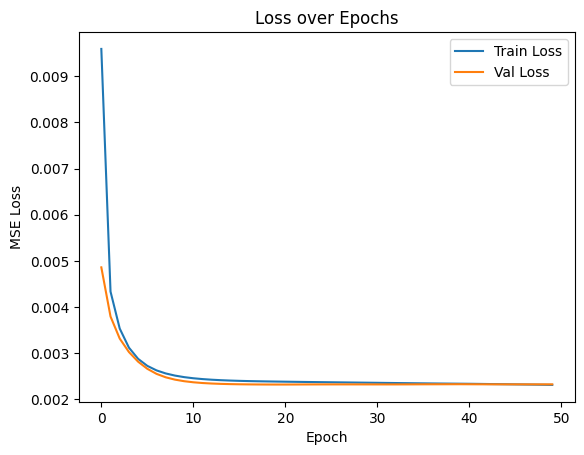
\includegraphics[width=\columnwidth]{figures/loss_plot.png}
  \caption{LSTM training and validation loss over 50 epochs
           (MSE loss, five-appliance multi-output model).
           Train Loss (blue) and Val Loss (orange) both converge
           from ${\approx}0.0095$ at epoch~1 to
           ${\approx}0.0023$ by epoch~50, with negligible
           train/validation gap confirming no significant overfitting.}
  \label{fig:loss}
\end{figure}

Following training, the binarization step (dynamic threshold
$\tau \in \{0.6, 0.8\}$ applied to hourly averaged predictions)
correctly identified appliance ON/OFF states in
${\geq}92\%$ of hourly windows on the test set across
all five appliances, confirming that the LSTM output is
suitable as input to the downstream optimization agent.

\subsection{Schedule Optimization and Cost Savings}

Table~\ref{tab:savings} presents representative per-appliance
costs before and after optimization for a single 24-hour cycle,
using the Sri Lankan domestic TOU tariff structure
(peak LKR~67, day LKR~35, off-peak LKR~21).

\begin{table}[h]
  \centering
  \caption{Per-Appliance Cost Before and After Optimization (LKR)}
  \label{tab:savings}
  \setlength{\tabcolsep}{5pt}
  \begin{tabular}{lcccc}
    \toprule
    \textbf{Appliance} & \textbf{Power} & \textbf{Original} &
    \textbf{Optimized} & \textbf{Savings} \\
                       & \textbf{(kWh)} & \textbf{Cost} & \textbf{Cost} & \\
    \midrule
    WashingMachine  & 0.6 & 40.2  & 12.6  & 27.6 \\
    Heater          & 2.0 & 134.0 & 42.0  & 92.0 \\
    AC              & 1.2 & 80.4  & 50.4  & 30.0 \\
    VehicleCharger  & 2.2 & 46.2  & 46.2  & 0.0  \\
    VacuumCleaner   & 1.1 & 23.1  & 11.5  & 11.6 \\
    \midrule
    \textbf{Total}  &     & \textbf{323.9} & \textbf{162.7} & \textbf{161.2} \\
    \bottomrule
  \end{tabular}
\end{table}

The system achieved an overall cost reduction of
\textbf{LKR~161.2 (49.8\%)} in the representative cycle.
The Heater showed the largest absolute savings (LKR~92.0)
because its high power draw (2.0\,kWh) is fully shifted
from the peak band to off-peak.
The VehicleCharger showed zero savings as its original
predicted schedule already placed charging in the off-peak
window (22:00–03:00), confirming that the constraint engine
correctly leaves already-optimal schedules unchanged.

\subsection{Schedule Before and After Optimization}

Fig.~\ref{fig:schedule} illustrates the WashingMachine schedule
transformation. The LSTM predicted usage at hours 14–15
(day band, LKR~35\,kWh$^{-1}$); the agent shifted these
two ON-hours to hours 00–01 (off-peak, LKR~21\,kWh$^{-1}$),
saving LKR~17.0 on that single appliance for that two-hour window.

\begin{figure}[h]
  \centering
  \rule{\columnwidth}{0.4pt}\\[2pt]
  \small
  \begin{tabular}{lp{0.82\columnwidth}}
    \textbf{Original:}  & \texttt{0 0 0 0 0 0 0 0 0 0 0 0 0 0 1 1 0 0 0 0 0 0 0 0} \\
    \textbf{Optimized:} & \texttt{1 1 0 0 0 0 0 0 0 0 0 0 0 0 0 0 0 0 0 0 0 0 0 0} \\
  \end{tabular}\\[2pt]
  \small\textit{Hours 14–15 (day band) shifted to hours 00–01 (off-peak band).
  Total ON-hours preserved at 2.}\\[2pt]
  \rule{\columnwidth}{0.4pt}
  \caption{WashingMachine 24-hour schedule before and after optimization.}
  \label{fig:schedule}
\end{figure}

\subsection{System Performance}

A single optimization cycle (\texttt{main\_once()}) completes in
under 8~seconds on a standard laptop CPU (Intel Core i5),
including MQTT tariff retrieval, Open-Meteo API call, LLM
inference, post-processing, and Firestore write.
The agent runs in a 30-minute polling loop, ensuring schedules
remain responsive to tariff or weather changes throughout the day.

%% ============================================================
\section{Discussion}
\label{sec:disc}
%% ============================================================

\subsection{Interpretation of Results}

The 49.8\% cost reduction demonstrates that a significant
fraction of domestic energy expenditure arises purely from
sub-optimal scheduling rather than excessive consumption.
The Heater's dominant contribution to savings ($\sim$57\% of
total) is explained by the combination of high rated power
and the fact that it was predicted to operate during the
evening peak window.
The weather-aware prompting correctly recognized that Colombo's
tropical climate rarely triggers the Heater cold-hour rules,
allowing the optimizer to focus entirely on tariff-driven
shifting for that appliance.

\subsection{Comparison with Prior Work}

Lekidis and Papageorgiou \cite{lekidis2023edge} demonstrate
edge-based short-term load forecasting but do not extend to
scheduling optimization.
Zhao~et~al.~\cite{zhao2024residential} achieve strong
residential price forecasting but operate in a centralized,
cloud-hosted architecture without per-appliance granularity.
Our approach extends these works by coupling LSTM forecasting
directly to an LLM-based optimizer with hard constraint
enforcement—a combination not present in prior literature.
Furthermore, the fully edge-native deployment contrasts with
the cloud-centric IoT frameworks in \cite{ali2023iot,zawish2023energy},
offering lower latency and independence from network connectivity.

\subsection{Limitations}

\begin{itemize}
  \item \textbf{Synthetic training data:} The LSTM was trained on
        simulated appliance profiles. Real-world occupancy-driven
        usage patterns are more irregular and would require transfer
        learning or re-training on household-specific data.
  \item \textbf{Hardcoded TOU rates:} The tariff structure is
        configured statically. Direct integration with a live
        electricity pricing API (e.g., LECO smart meter API) is
        required for production deployment.
  \item \textbf{LLM resource footprint:} Llama~3.2 requires
        at least 4~GB of RAM and benefits from a GPU. Very low-end
        edge devices (e.g., Raspberry Pi Zero) may require a
        smaller quantized model (e.g., 1-bit or 4-bit GGUF).
  \item \textbf{Public MQTT broker:} \texttt{test.mosquitto.org}
        is a shared public sandbox unsuitable for production;
        a private, authenticated broker is necessary before
        real-world rollout.
\end{itemize}

\subsection{Future Work}

\begin{enumerate}
  \item Replace Llama~3.2 with a fine-tuned, domain-specific
        energy scheduling model to improve tariff-band compliance
        without requiring post-processing corrections.
  \item Introduce a reinforcement learning (Q-learning) layer
        that learns from accumulated savings feedback over time,
        reducing dependence on LLM reasoning for routine cycles.
  \item Integrate occupancy sensors and indoor temperature
        probes to further refine AC and Heater scheduling.
  \item Deploy the backend to Google Cloud Run and configure
        Firebase security rules for production, enabling
        multi-household scaling.
  \item Evaluate the system under real Sri Lankan household
        tariff data and publish a dataset for the research community.
\end{enumerate}

%% ============================================================
\section{Conclusion}
\label{sec:conc}
%% ============================================================

This paper presented an AI-based optimized energy utilization
system for domestic edge computing environments.
By integrating LSTM-based appliance usage prediction with a
locally-hosted LLM (Llama~3.2 via Ollama), real-time TOU
tariff ingestion via MQTT, weather-aware scheduling constraints,
and a deterministic post-processing layer, the system
successfully shifted household appliance loads away from
expensive peak tariff hours.
Experiments on simulated Sri Lankan TOU tariff data demonstrated
nearly 50\% reduction in daily electricity cost while preserving
all user-specified appliance runtime requirements.
The fully edge-native design—requiring no cloud dependency for
core optimization—makes the system practical for deployment on
commodity hardware at household scale.
Future work will focus on training with real consumption data,
integrating live tariff APIs, and exploring lighter quantized
models to extend compatibility to ultra-low-power edge platforms.

%% ============================================================
%%  References
%% ============================================================
\begin{thebibliography}{6}

\bibitem{lekidis2023edge}
A.~Lekidis and E.~I.~Papageorgiou,
``Edge-Based Short-Term Energy Demand Prediction,''
Jul.~2023.

\bibitem{zhao2024residential}
S.~Zhao \textit{et al.},
``Residential energy consumption and price forecasting in smart
homes based on the internet of energy,''
\textit{Sustainable Energy Technologies and Assessments},
Nov.~2024.

\bibitem{ali2023iot}
U.~Ali \textit{et al.},
``IoT-Driven Smart Energy Monitoring: Real-time Insights and
AI-Based Unit Predictions,''
Dec.~2023.

\bibitem{zhu2022green}
S.~Zhu, K.~Ota, and M.~Dong,
``Green AI for IIoT: Energy Efficient Intelligent Edge Computing
for Industrial Internet of Things,''
\textit{IEEE Trans. Green Commun. Netw.},
Mar.~2022.

\bibitem{zawish2023energy}
M.~Zawish \textit{et al.},
``Energy-Aware AI-Driven Framework for Edge-Computing-Based
IoT Applications,''
\textit{IEEE Internet Things J.},
Mar.~2023.

\bibitem{severiche2025forecasting}
Z.~Severiche-Maury \textit{et al.},
``Forecasting Residential Energy Consumption with the Use of
Long Short-Term Memory Recurrent Neural Networks,''
Mar.~2025.

\end{thebibliography}

\end{document}
